\begin{figure}
	\centering
	\subcaptionbox{\label{fig:disoTPS_TEBD_five_tensor_environment}}
	{%
		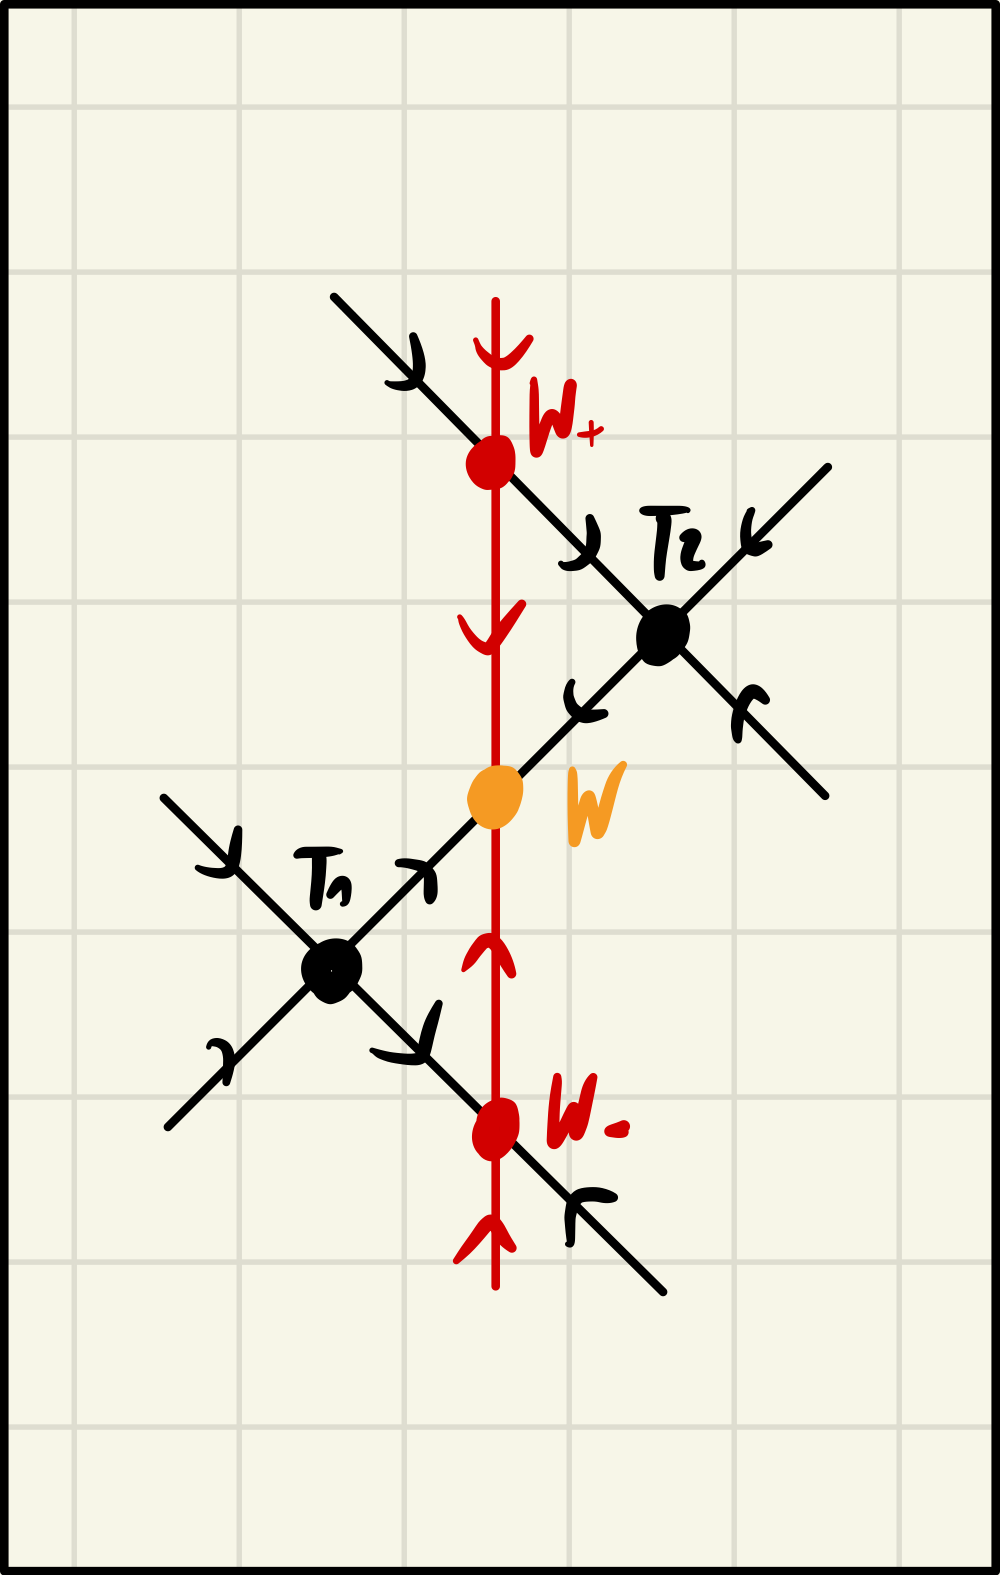
\includegraphics[width=0.3\textwidth]{figures/disoTPS/disoTPS_TEBD_5_tensor_environment.jpeg}
	}
	\subcaptionbox{\label{fig:disoTPS_TEBD_contraction_definition}}
	{%
		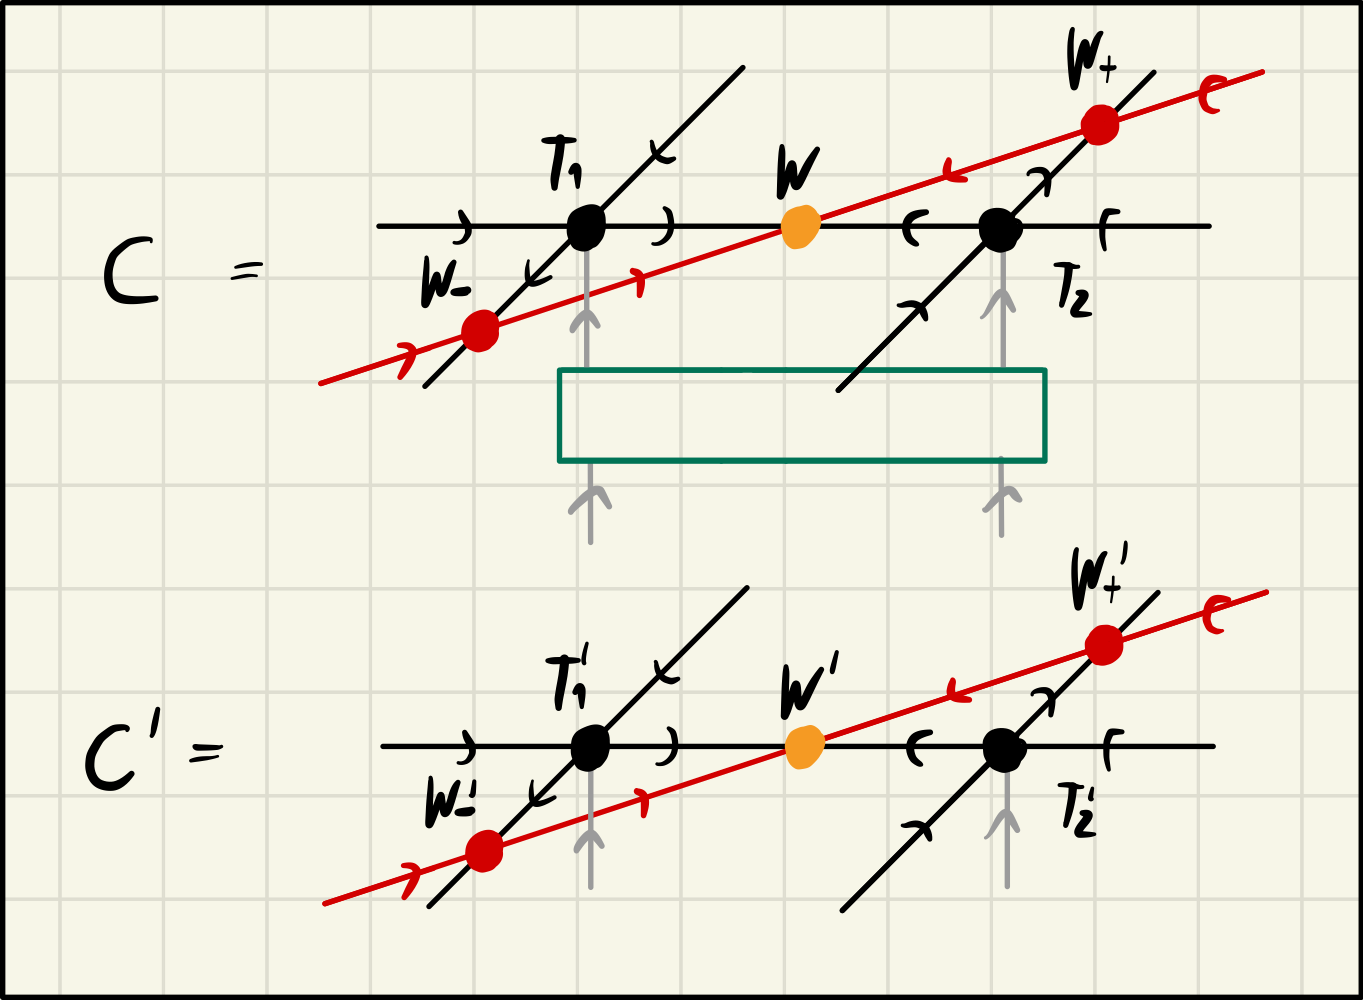
\includegraphics[width=0.6\textwidth]{figures/disoTPS/disoTPS_TEBD_contraction_definitions.jpeg}
	}
	\caption{(a The five tensor environment of the bond on which the bond operator is to be applied. All arrows are incoming. (b) Definitions of the sub-networks $\mathcal{C}$ and $\mathcal{C}^\prime$ used in equation \eqref{eq:isoDTPS_TEBD_local_update_error}.}
	\label{fig:disoTPS_TEBD_definition_of_environment}
\end{figure}
Let us assume that the orthogonality center is positioned between the two sites on which the bond operator $\hat{U}^{[x, y]}\left(\Delta t\right)$ acts. The five tensors around the orthogonality center then make up a sub-network with only incoming arrows, see figure \figref{fig:disoTPS_TEBD_five_tensor_environment}. We call these five tensors $T_1$, $T_2$, $W_1$, $W_2$ and $W_3$. The local TEBD update can then be formulated as the following problem: Find tensors $T_1^\prime$, $T_2^\prime$, $W_1^\prime$, $W_2^\prime$ and $W_3^\prime$ satisfying the isometry constraints and minimizing the error
\begin{equation}
	\label{eq:isoDTPS_TEBD_local_update_error}
	\varepsilon_\text{trunc} = \left\lVert \hat{U}^{[x,y]}(\Delta t)|\Psi\rangle - |\Psi\rangle\right\rVert = \underset{T_1^\prime, T_2^\prime, W_1^\prime, W_2^\prime, W_3^\prime}{\argmax}\Re\langle\mathcal{C}|\mathcal{C}^\prime\rangle_\text{F}.
\end{equation}
The tensors $\mathcal{C}$ and $\mathcal{C}^\prime$ denote the contracted sub-networks that are defined in figure \figref{fig:disoTPS_TEBD_contraction_definition}. For solving this problem we use the Evenbly-Vidal algorithm, inspired by \cite{cite:fast_time_evolution_of_mps_using_qr}, where a similar algorithm was used to speed up TEBD for MPS. As we already did in section \ref{sec:YB_move_iterative_local_optimization} for the YB move, we optimize one tensor at a time while keeping all other tensors fixed. This procedure is then repeated, sweeping over all five tensors until convergence is achieved. For more details on this optimization method see appendix \ref{app:riemannian_optimization_of_isometries}. One iteration of the algorithm is shown in figure \figref{fig:disoTPS_TEBD_local_update_detailed}.
\begin{figure}
	\centering
	\subcaptionbox{\label{fig:disoTPS_TEBD_local_update_T1}}
	{%
		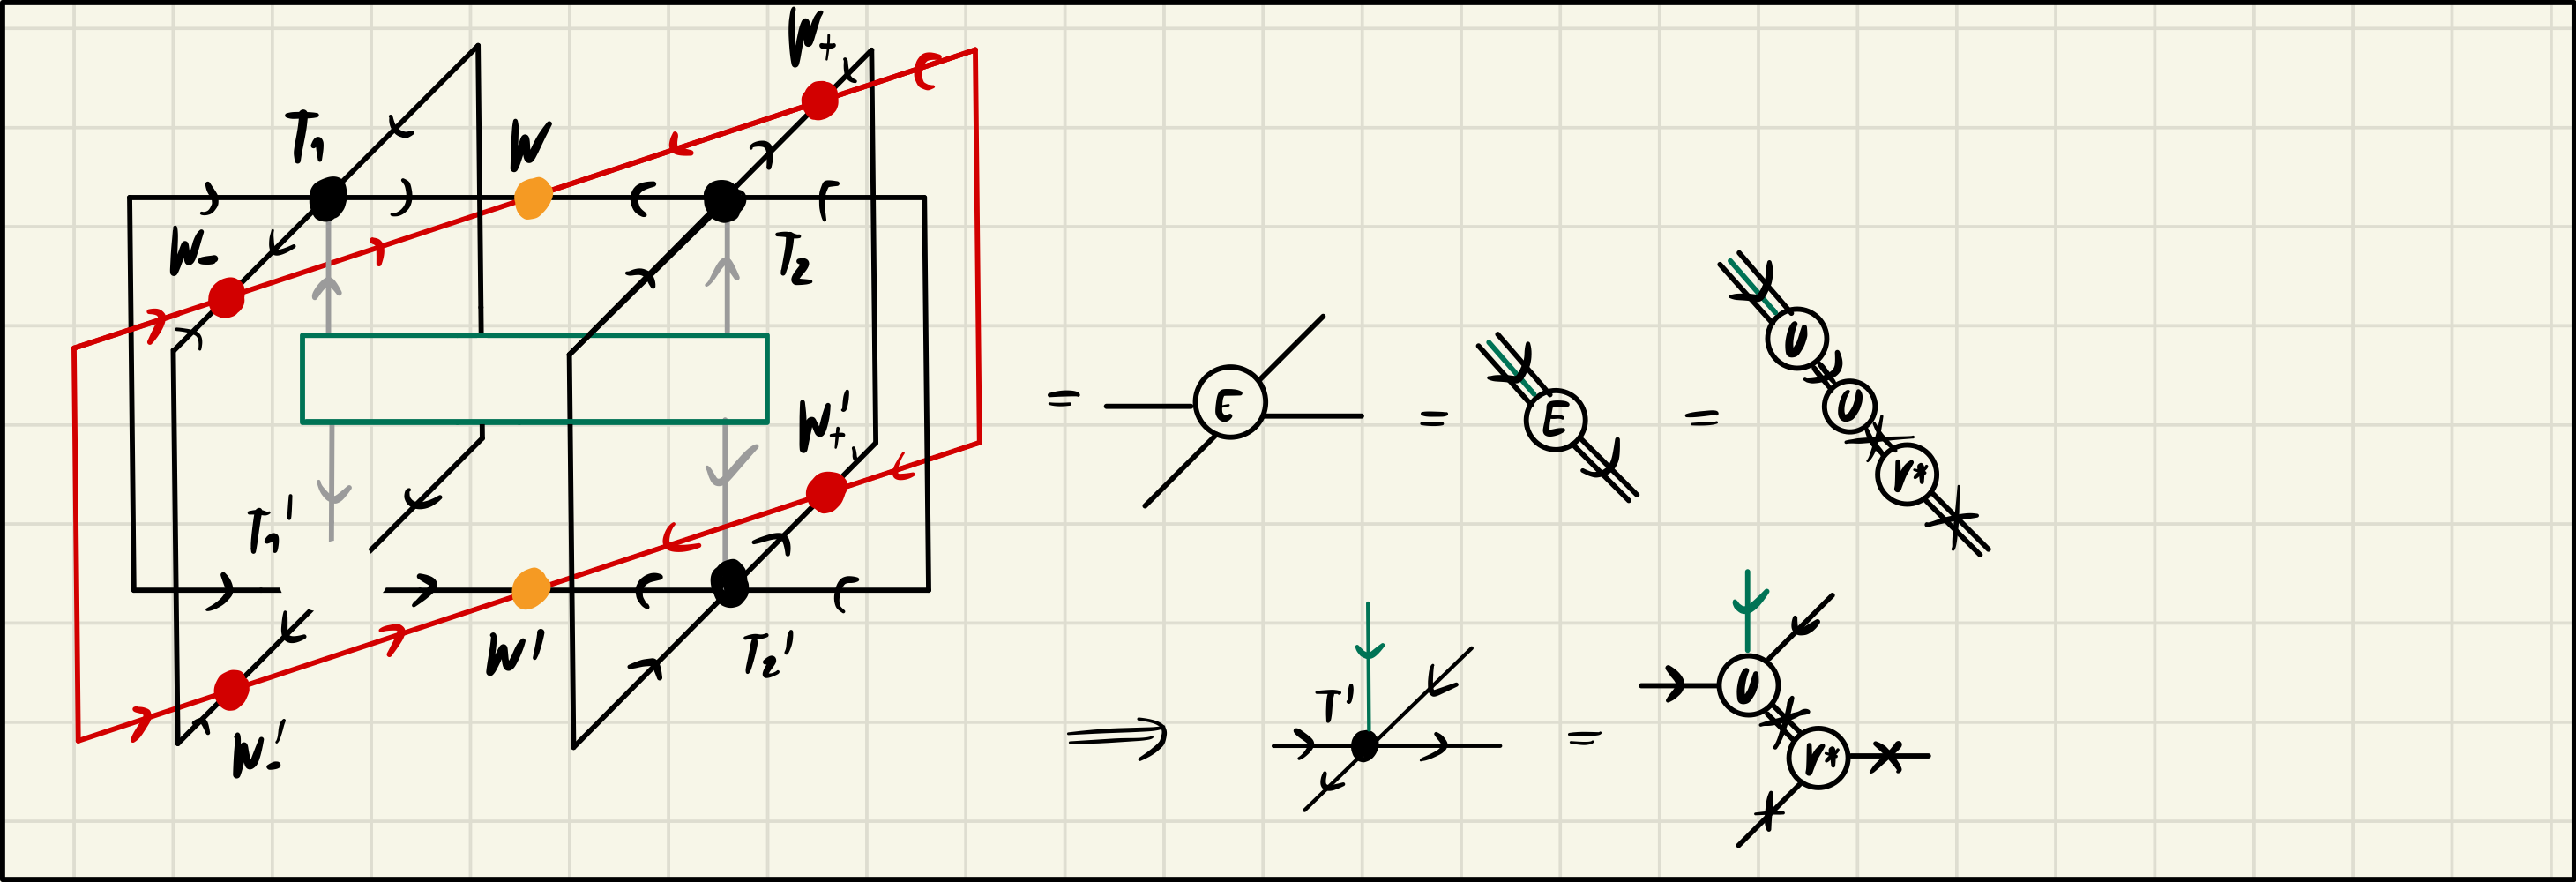
\includegraphics[width=0.6\textwidth]{figures/disoTPS/disoTPS_TEBD_local_update_T1.jpeg}
	}
	\subcaptionbox{\label{fig:disoTPS_TEBD_local_update_W1}}
	{%
		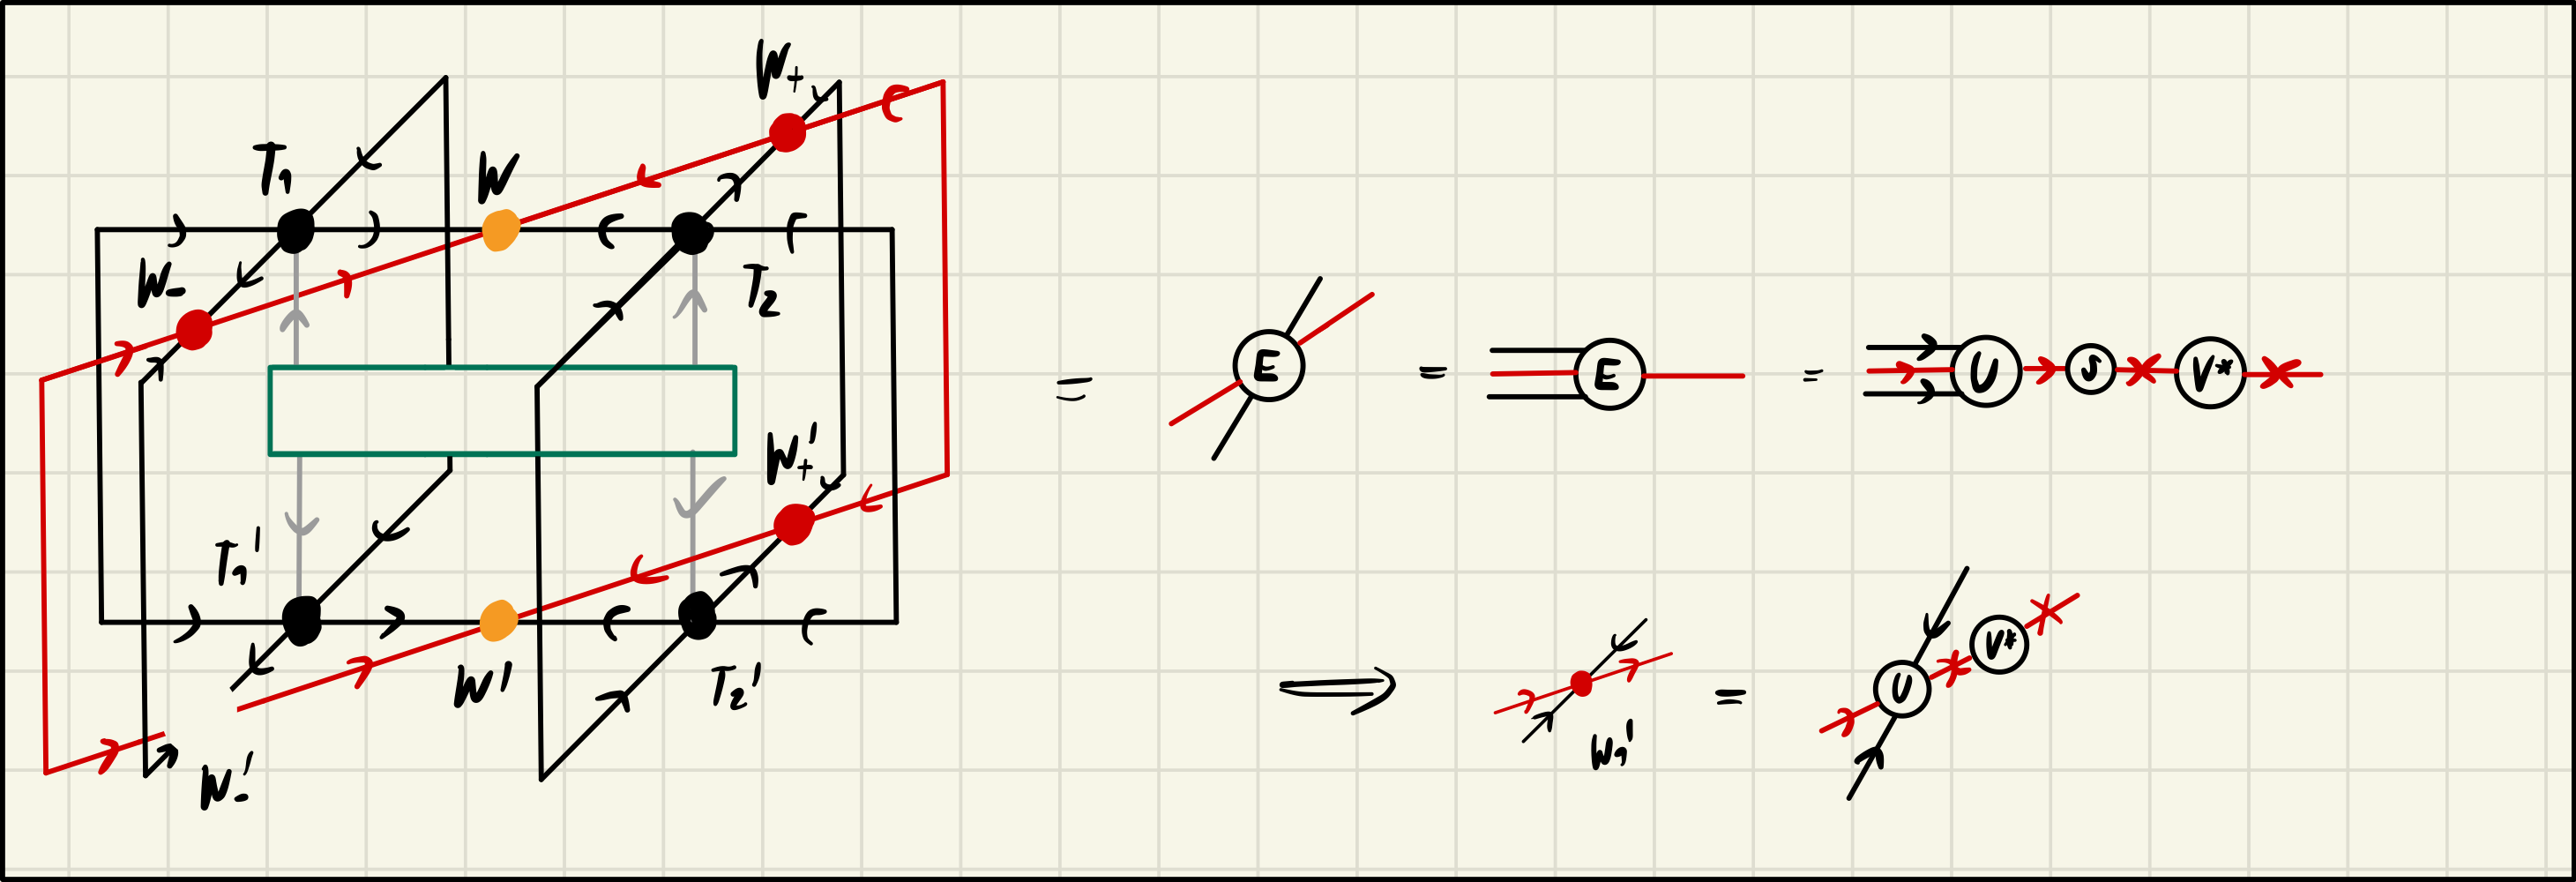
\includegraphics[width=0.6\textwidth]{figures/disoTPS/disoTPS_TEBD_local_update_Wm.jpeg}
	}
	\subcaptionbox{\label{fig:disoTPS_TEBD_local_update_T2}}
	{%
		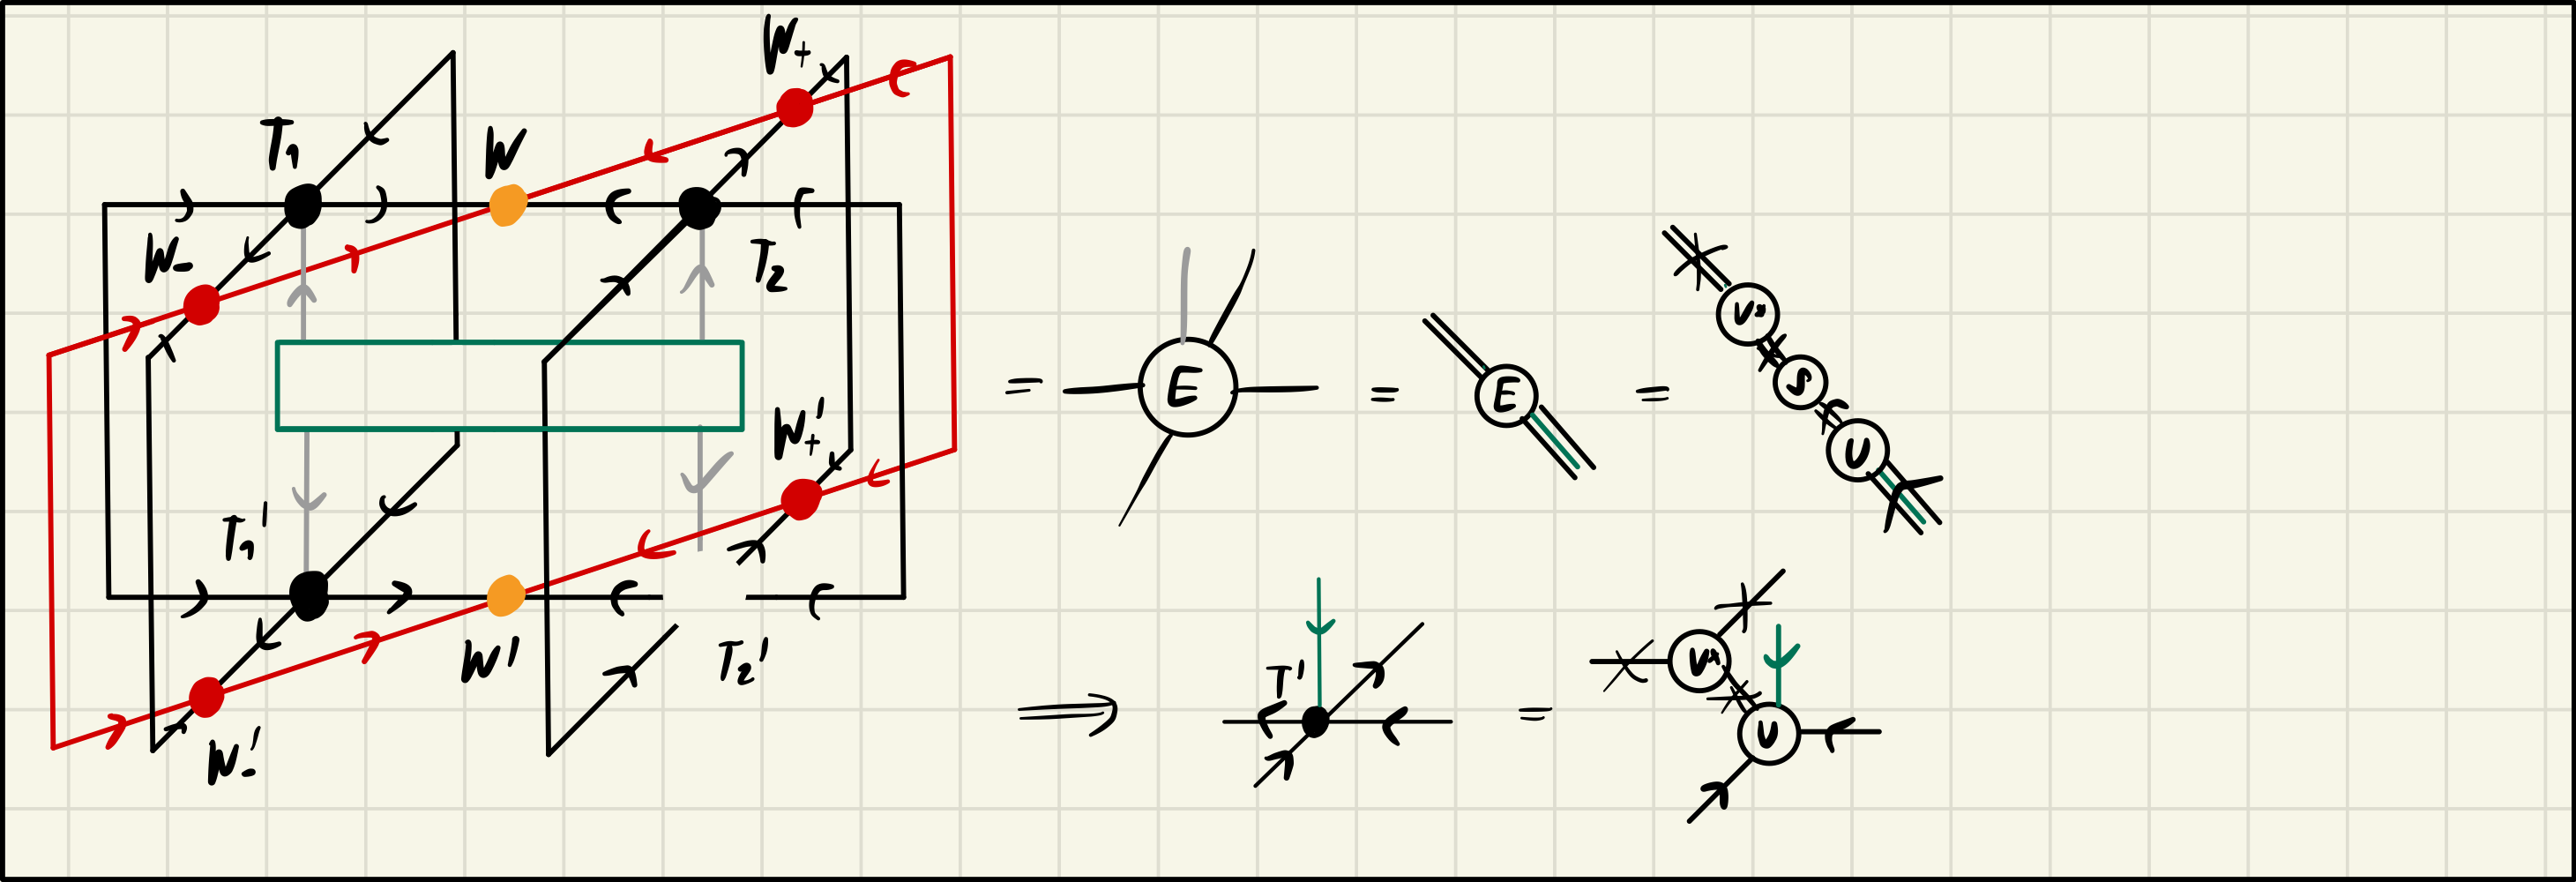
\includegraphics[width=0.6\textwidth]{figures/disoTPS/disoTPS_TEBD_local_update_T2.jpeg}
	}
	\subcaptionbox{\label{fig:disoTPS_TEBD_local_update_W3}}
	{%
		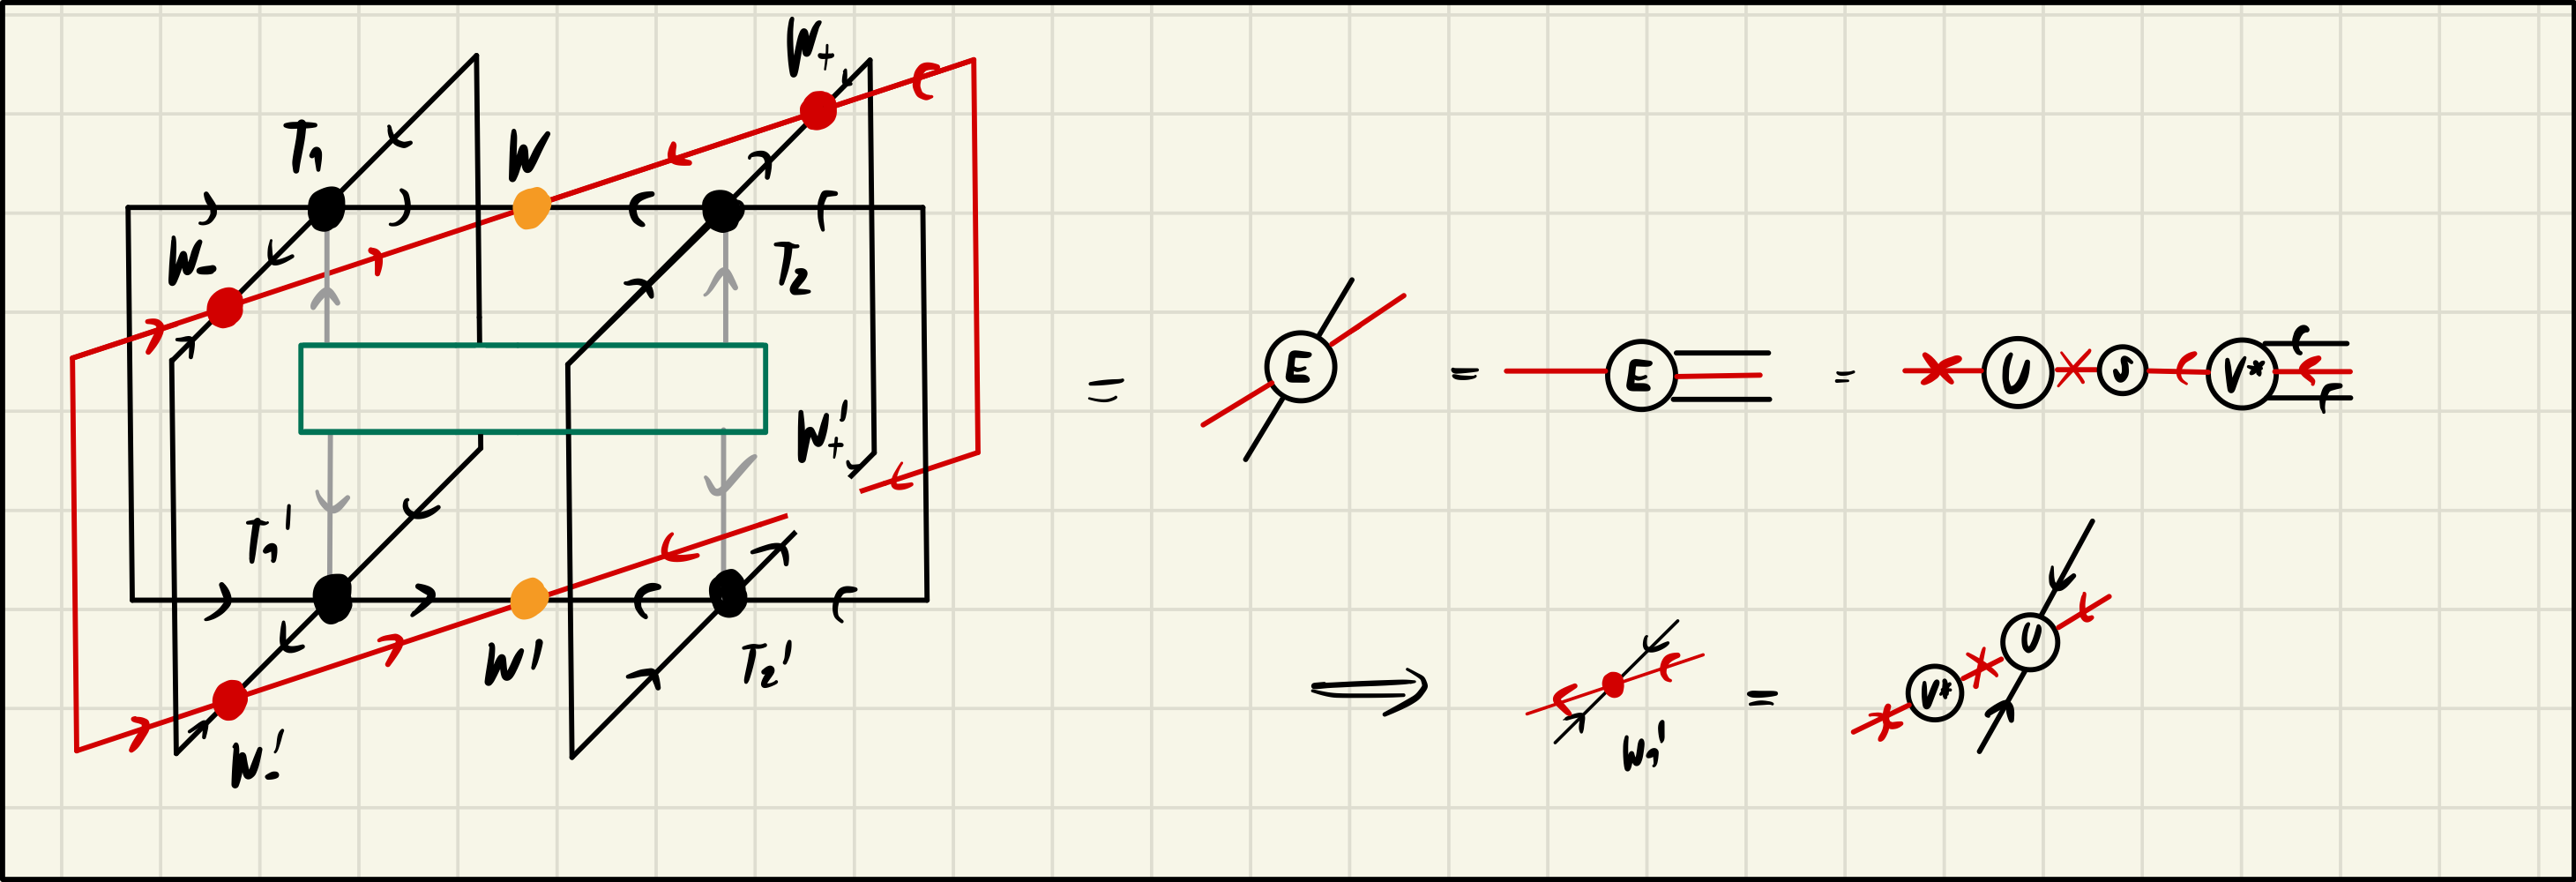
\includegraphics[width=0.6\textwidth]{figures/disoTPS/disoTPS_TEBD_local_update_Wp.jpeg}
	}
	\subcaptionbox{\label{fig:disoTPS_TEBD_local_update_W2}}
	{%
		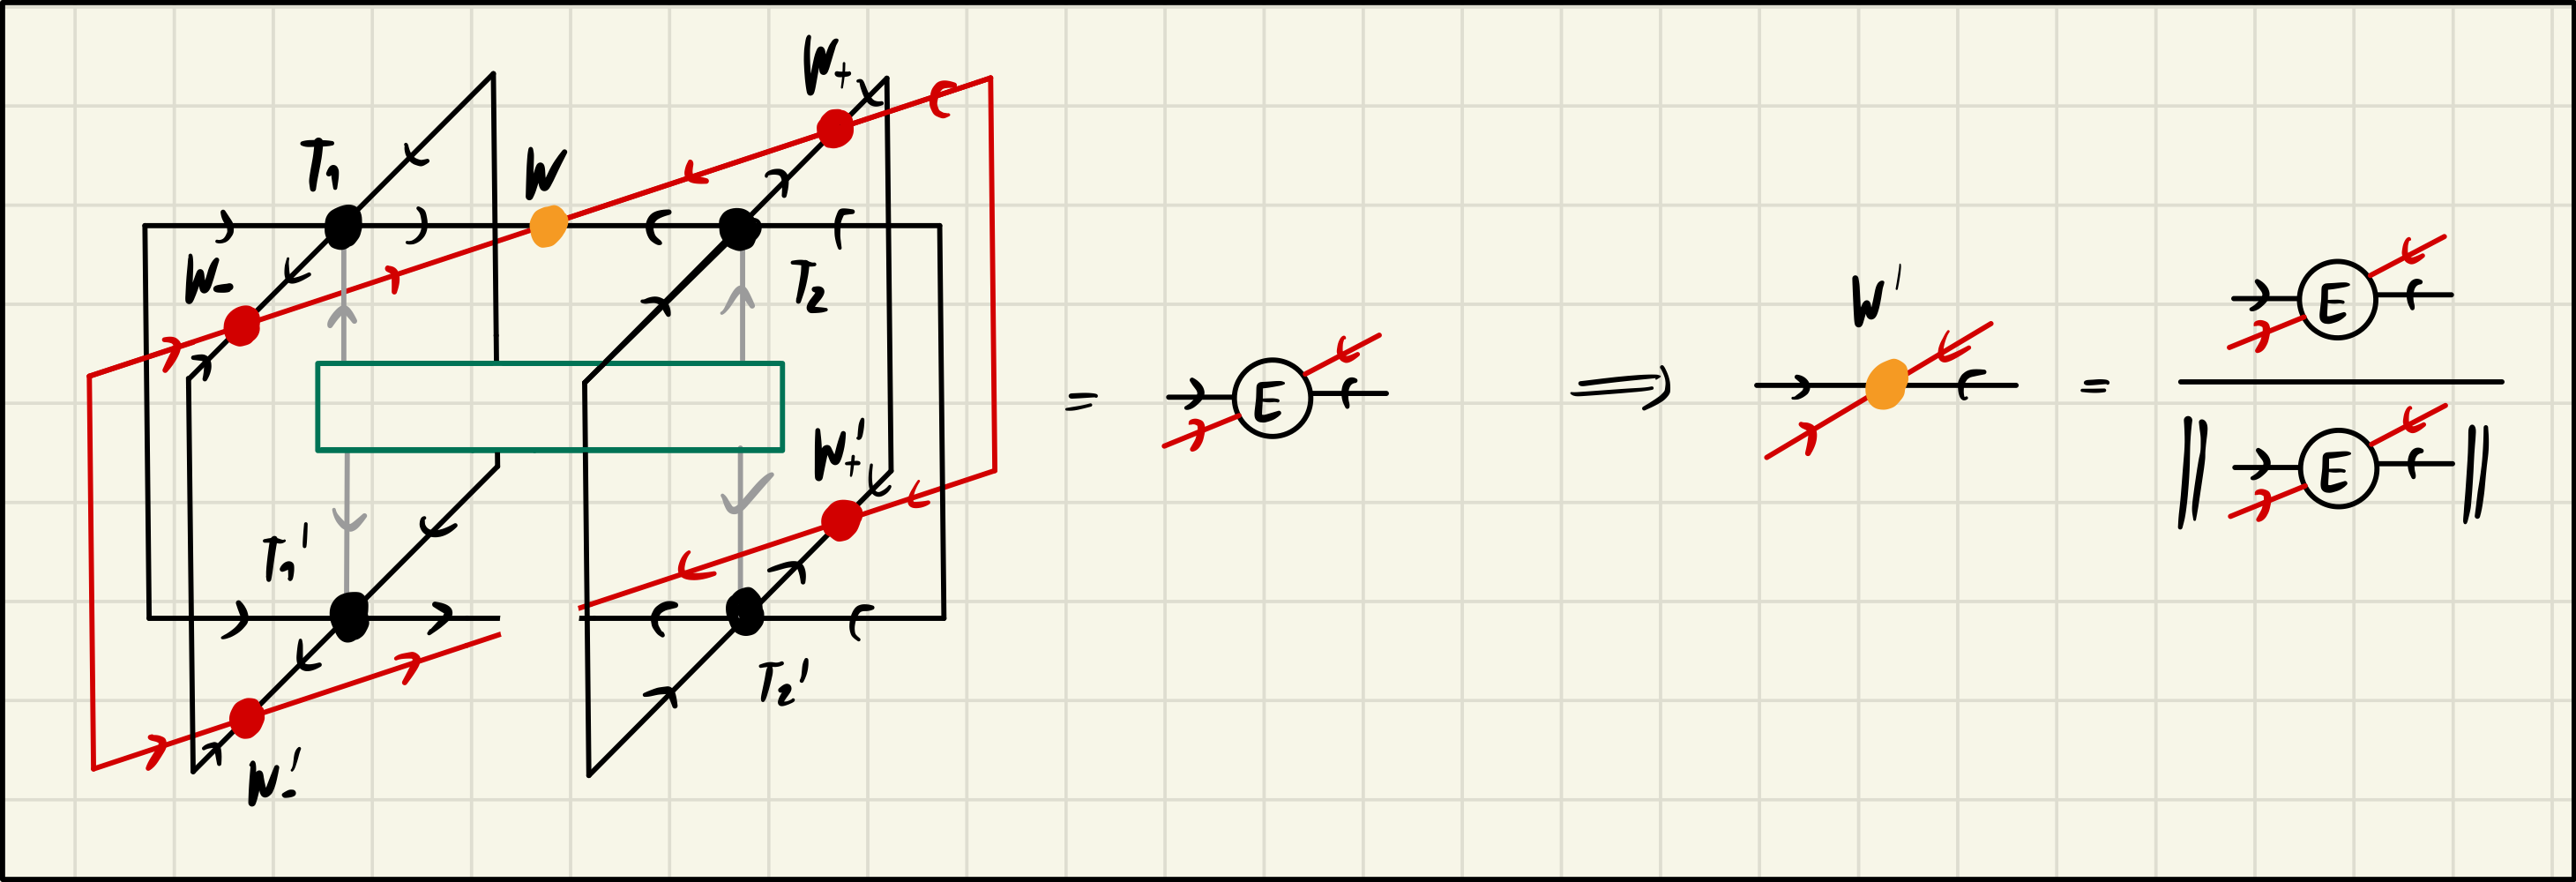
\includegraphics[width=0.6\textwidth]{figures/disoTPS/disoTPS_TEBD_local_update_W.jpeg}
	}
	\caption{A local TEBD update can be applied by variational optimization of five tensors. Subfigures (a)-(e) show steps 1-5 of one iteration of the algorithm, updating each tensor once.}
	\label{fig:disoTPS_TEBD_local_update_detailed}
\end{figure}
